\documentclass[12pt,a4paper]{article}

% ================= PAQUETES =================
\usepackage[utf8]{inputenc}
\usepackage[T1]{fontenc}
\usepackage{newtxtext,newtxmath}
\usepackage[top=2.5cm, bottom=2.5cm, left=3.5cm, right=2.5cm]{geometry}
\usepackage{setspace}
\doublespacing
\usepackage{graphicx}
\usepackage{indentfirst}
\usepackage[hidelinks]{hyperref}
\usepackage{titlesec}
\usepackage{caption}
\usepackage{booktabs}
\usepackage{multirow}
\usepackage{array}
\usepackage{enumitem}
\usepackage{amsmath}
\usepackage{longtable}
\usepackage{float}
\usepackage{tabularx}

% ================= COLORES PARA TABLAS =================
\usepackage[table]{xcolor}

% ================= ALGORITMOS Y PSEUDOCÓDIGO =================
\usepackage[ruled,vlined,onelanguage]{algorithm2e}
\SetKwComment{Comment}{// }{}
\SetKwInput{KwInput}{Entrada}
\SetKwInput{KwOutput}{Salida}
\SetKwFor{ForEach}{para cada}{hacer}{fin para}
\SetKwIF{Si}{SinoSi}{Sino}{si}{entonces}{sino si}{sino}{fin si}
\SetKwFor{Para}{para}{hacer}{fin para}
\SetKwFor{While}{mientras}{hacer}{fin mientras}
\SetKwProg{Fn}{Función}{:}{fin}

% ================= SUBFIGURAS =================
\usepackage{subcaption}

% ================= FORMATO DE TÍTULOS =================
\titleformat{\section}{\normalfont\Large\bfseries\centering}{\thesection.}{1em}{\MakeUppercase}
\titleformat{\subsection}{\normalfont\large\bfseries}{\thesubsection.}{1em}{\MakeUppercase}
\titleformat{\subsubsection}{\normalfont\normalsize\bfseries}{\thesubsubsection.}{1em}{}

% ================= FORMATO DE TABLAS Y FIGURAS =================
\captionsetup[table]{labelsep=newline, textfont=it, font=normalsize, justification=raggedright, singlelinecheck=off}
\captionsetup[figure]{labelsep=newline, textfont=it, font=normalsize, justification=raggedright, singlelinecheck=off}

% ================= PÁRRAFOS =================
\setlength{\parindent}{1.25cm}
\setlength{\parskip}{10pt}

\usepackage[spanish,es-tabla]{babel}

\begin{document}

% ================= CARÁTULA =================
\begin{titlepage}
    \centering
    \setlength{\parindent}{0pt}
    \setlength{\parskip}{0pt}

    {\fontsize{18}{21}\selectfont \textbf{UNIVERSIDAD NACIONAL DEL ALTIPLANO} \par}
    \vspace{0.5cm}
    {\fontsize{16}{19}\selectfont \textbf{FACULTAD DE INGENIERÍA DE MECÁNICA ELÉCTRICA, ELECTRÓNICA Y SISTEMAS} \par}
    \vspace{0.3cm}
    {\fontsize{14}{17}\selectfont \textbf{ESCUELA PROFESIONAL DE INGENIERÍA DE SISTEMAS} \par}

    \vspace{1cm}
    %
\includegraphics[width=4.33cm, height=4.68cm]{../logo_unap.png}
    \vspace{1cm}

    {\fontsize{14}{17}\selectfont \textbf{CURSO:} \par}
    {\fontsize{14}{17}\selectfont LENGUAJES DE PROGRAMACIÓN \par}

    \vspace{1cm}
    {\fontsize{14}{17}\selectfont \textbf{TÍTULO DEL PROYECTO:} \par}
    {\fontsize{14}{17}\selectfont \textbf{Árboles de Dependencia, Información Mutua y Redes Bayesianas \\ Predicción de Abandono Universitario} \par}

    \vspace{1cm}
    {\fontsize{14}{17}\selectfont \textbf{DOCENTE:} \par}
    {\fontsize{14}{17}\selectfont ING. JUARES RUELAS JOSE LUIS \par}

    \vspace{1cm}
    {\fontsize{14}{17}\selectfont \textbf{PRESENTADO POR:} \par}
    {\fontsize{16}{19}\selectfont \textbf{JAHUIRA PONCE CHRISTIAN SEBASTIÁN} \par}

    \vfill
    {\fontsize{14}{17}\selectfont \textbf{PUNO -- PERÚ} \par}
    {\fontsize{14}{17}\selectfont \textbf{2026} \par}
\end{titlepage}

\newpage
\tableofcontents
\newpage

% ================= ENLACE =================
\thispagestyle{empty}
\begin{center}
    \textbf{Repositorio del Proyecto}\\
    \url{https://github.com/HidenXye/Lenguajes-Split}
\end{center}
\newpage

% =============================================
% INTRODUCCIÓN
% =============================================
\section{Introducción}

El presente proyecto extiende el análisis de árboles de dependencia basados en Información Mutua (IM) al dataset \texttt{Predict Students' Dropout and Academic Success} (Realinho et al., 2021), obtenido del UCI Machine Learning Repository (Dataset ID: 697). Este dataset contiene registros reales de 4,424 estudiantes de una institución de educación superior en Portugal, con información demográfica, socioeconómica y de rendimiento académico.

Se seleccionaron 9 variables predictoras más la variable objetivo \texttt{Target} (abandono, inscrito o graduado). Como criterio de partición se emplea la variable \texttt{Displaced} (estudiante desplazado de su residencia habitual), generando dos subconjuntos independientes:

\begin{itemize}
    \item \textbf{Dataset A}: Estudiantes \textbf{no desplazados} (1,998 filas).
    \item \textbf{Dataset B}: Estudiantes \textbf{desplazados} (2,426 filas).
\end{itemize}

En cada subconjunto se elimina la variable de partición y se trabaja con 10 columnas: 9 variables predictoras y la variable objetivo. Para cada dataset se repite el procedimiento completo: cálculo de entropía individual, matriz de información mutua, construcción del Árbol de Expansión de Peso Máximo (MST) mediante los algoritmos de Kruskal y Prim, visualización del grafo resultante, y análisis de sensibilidad mediante el método rVP. Adicionalmente, se extiende el análisis al aprendizaje de una Red Bayesiana mediante el algoritmo de Chow-Liu.

\subsection{Variables del análisis}

\begin{table}[H]
    \centering
    \begin{tabular}{cll}
        \toprule
        \textbf{Variable} & \textbf{Descripción} & \textbf{Tipo} \\
        \midrule
        $x_1$ & Nota de admisión & Ordinal (0, 1, 2) \\
        $x_2$ & Edad al ingreso & Ordinal (0, 1, 2) \\
        $x_3$ & Pagos al día & Binaria \\
        $x_4$ & Becado & Binaria \\
        $x_5$ & Aprobados 1er semestre & Ordinal (0, 1, 2) \\
        $x_6$ & Nota media 1er semestre & Ordinal (0, 1, 2) \\
        $x_7$ & Aprobados 2do semestre & Ordinal (0, 1, 2) \\
        $x_8$ & Nota media 2do semestre & Ordinal (0, 1, 2) \\
        $x_9$ & Estado civil & Binaria (soltero/otro) \\
        \midrule
        \textbf{Target} & Abandono / Inscrito / Graduado & Categórica (3) \\
        \midrule
        \textbf{Split} & Desplazado & Binaria (Sí / No) \\
        \bottomrule
    \end{tabular}
    \caption{Variables seleccionadas para el análisis (9 predictoras + 1 objetivo).}
\end{table}

% =============================================
% DATASET A (NO DESPLAZADOS)
% =============================================
\section{Dataset A -- No Desplazados (1,998 registros)}

\subsection{Desarrollo de Entropía}

Se emplea la fórmula de Entropía de Shannon:
\begin{equation}
    H(X) = -\sum_{x \in X} p(x)\log_2(p(x))
\end{equation}

\subsubsection{Cálculo para $x_1$ (Nota de admisión)}
Probabilidades: $p(0) = \frac{736}{1998} = 0.3684$, $p(1) = \frac{621}{1998} = 0.3108$, $p(2) = \frac{641}{1998} = 0.3208$
\begin{align*}
    H(x_1) &= -\big[ (0.3684 \cdot \log_2(0.3684)) + (0.3108 \cdot \log_2(0.3108)) + (0.3208 \cdot \log_2(0.3208)) \big] \\
    H(x_1) &= -\big[ (0.3684 \cdot -1.4404) + (0.3108 \cdot -1.6859) + (0.3208 \cdot -1.6403) \big] \\
    H(x_1) &= 0.5306 + 0.5240 + 0.5262 = \textbf{1.5773}
\end{align*}

\subsubsection{Cálculo para $x_2$ (Edad)}
Probabilidades: $p(0) = \frac{724}{1998} = 0.3624$, $p(1) = \frac{511}{1998} = 0.2558$, $p(2) = \frac{763}{1998} = 0.3819$
\begin{align*}
    H(x_2) &= -\big[ (0.3624 \cdot \log_2(0.3624)) + (0.2558 \cdot \log_2(0.2558)) + (0.3819 \cdot \log_2(0.3819)) \big] \\
    H(x_2) &= 0.5303 + 0.5043 + 0.5291 = \textbf{1.4795}
\end{align*}

\subsubsection{Cálculo para $x_3$ (Pagos al día)}
Probabilidades: $p(0) = \frac{259}{1998} = 0.1296$, $p(1) = \frac{1739}{1998} = 0.8704$
\begin{align*}
    H(x_3) &= -\left[ (0.1296 \cdot \log_2(0.1296)) + (0.8704 \cdot \log_2(0.8704)) \right] \\
    H(x_3) &= -\left[ (0.1296 \cdot -2.9475) + (0.8704 \cdot -0.2002) \right] \\
    H(x_3) &= 0.3820 + 0.1742 = \textbf{0.6189}
\end{align*}

\subsubsection{Cálculo para $x_4$ (Becado)}
Probabilidades: $p(0) = \frac{1390}{1998} = 0.6957$, $p(1) = \frac{608}{1998} = 0.3043$
\begin{align*}
    H(x_4) &= -\left[ (0.6957 \cdot \log_2(0.6957)) + (0.3043 \cdot \log_2(0.3043)) \right] \\
    H(x_4) &= 0.3131 + 0.5206 = \textbf{0.7485}
\end{align*}

\subsubsection{Cálculo para $x_5$ (1er sem. aprobados)}
Probabilidades: $p(0) = \frac{780}{1998} = 0.3904$, $p(1) = \frac{827}{1998} = 0.4139$, $p(2) = \frac{391}{1998} = 0.1957$
\begin{align*}
    H(x_5) &= -\big[ (0.3904 \cdot \log_2(0.3904)) + (0.4139 \cdot \log_2(0.4139)) + (0.1957 \cdot \log_2(0.1957)) \big] \\
    H(x_5) &= 0.5294 + 0.5267 + 0.4600 = \textbf{1.4897}
\end{align*}

\subsubsection{Cálculo para $x_6$ (1er sem. nota)}
Probabilidades: $p(0) = \frac{675}{1998} = 0.3378$, $p(1) = \frac{651}{1998} = 0.3258$, $p(2) = \frac{672}{1998} = 0.3363$
\begin{align*}
    H(x_6) &= 0.5288 + 0.5276 + 0.5281 = \textbf{1.5724}
\end{align*}

\subsubsection{Cálculo para $x_7$ (2do sem. aprobados)}
Probabilidades: $p(0) = \frac{934}{1998} = 0.4675$, $p(1) = \frac{711}{1998} = 0.3559$, $p(2) = \frac{353}{1998} = 0.1767$
\begin{align*}
    H(x_7) &= -\big[ (0.4675 \cdot \log_2(0.4675)) + (0.3559 \cdot \log_2(0.3559)) + (0.1767 \cdot \log_2(0.1767)) \big] \\
    H(x_7) &= 0.5136 + 0.5297 + 0.4418 = \textbf{1.4851}
\end{align*}

\subsubsection{Cálculo para $x_8$ (2do sem. nota)}
Probabilidades: $p(0) = \frac{670}{1998} = 0.3353$, $p(1) = \frac{674}{1998} = 0.3373$, $p(2) = \frac{654}{1998} = 0.3273$
\begin{align*}
    H(x_8) &= 0.5286 + 0.5279 + 0.5280 = \textbf{1.5754}
\end{align*}

\subsubsection{Cálculo para $x_9$ (Estado civil)}
Probabilidades: $p(0) = \frac{1665}{1998} = 0.8333$, $p(1) = \frac{333}{1998} = 0.1667$
\begin{align*}
    H(x_9) &= -\left[ (0.8333 \cdot \log_2(0.8333)) + (0.1667 \cdot \log_2(0.1667)) \right] \\
    H(x_9) &= 0.2192 + 0.4308 = \textbf{0.7428}
\end{align*}

\subsubsection{Cálculo para Target}
Probabilidades: $p(0) = \frac{752}{1998} = 0.3764$, $p(1) = \frac{361}{1998} = 0.1807$, $p(2) = \frac{885}{1998} = 0.4429$
\begin{align*}
    H(Target) &= 0.5256 + 0.4462 + 0.5116 = \textbf{1.4970}
\end{align*}

\subsection{Matriz de Información Mutua}

La fórmula de IM es:
\begin{equation}
    IM(X,Y) = \sum_{x \in X}\sum_{y \in Y} p(x,y) \log_2 \left(\frac{p(x,y)}{p(x)p(y)}\right)
\end{equation}

\subsubsection{Ejemplo detallado: $x_7$ con Target}

Probabilidades marginales: $p(Target=0)=0.3764$, $p(Target=1)=0.1807$, $p(Target=2)=0.4429$, $p(x_7=0)=0.4675$, $p(x_7=1)=0.3559$, $p(x_7=2)=0.1767$.

\begin{align*}
    \text{Term. } (0,0) &= 0.3158 \cdot \log_2\left(\frac{0.3158}{0.4675 \cdot 0.3764}\right) = 0.3158 \cdot \log_2(1.7957) = \mathbf{+0.2665} \\
    \text{Term. } (0,1) &= 0.1071 \cdot \log_2\left(\frac{0.1071}{0.4675 \cdot 0.1807}\right) = 0.1071 \cdot \log_2(1.2678) = \mathbf{+0.0367} \\
    \text{Term. } (0,2) &= 0.0445 \cdot \log_2\left(\frac{0.0445}{0.4675 \cdot 0.4429}\right) = 0.0445 \cdot \log_2(0.2151) = \mathbf{-0.0987} \\
    \text{Term. } (1,0) &= 0.0445 \cdot \log_2\left(\frac{0.0445}{0.3559 \cdot 0.3764}\right) = 0.0445 \cdot \log_2(0.3324) = \mathbf{-0.0707} \\
    \text{Term. } (1,1) &= 0.0551 \cdot \log_2\left(\frac{0.0551}{0.3559 \cdot 0.1807}\right) = 0.0551 \cdot \log_2(0.8565) = \mathbf{-0.0123} \\
    \text{Term. } (1,2) &= 0.2563 \cdot \log_2\left(\frac{0.2563}{0.3559 \cdot 0.4429}\right) = 0.2563 \cdot \log_2(1.6256) = \mathbf{+0.1797} \\
    \text{Term. } (2,0) &= 0.0160 \cdot \log_2\left(\frac{0.0160}{0.1767 \cdot 0.3764}\right) = 0.0160 \cdot \log_2(0.2409) = \mathbf{-0.0329} \\
    \text{Term. } (2,1) &= 0.0185 \cdot \log_2\left(\frac{0.0185}{0.1767 \cdot 0.1807}\right) = 0.0185 \cdot \log_2(0.5797) = \mathbf{-0.0145} \\
    \text{Term. } (2,2) &= 0.1421 \cdot \log_2\left(\frac{0.1421}{0.1767 \cdot 0.4429}\right) = 0.1421 \cdot \log_2(1.8161) = \mathbf{+0.1224}
\end{align*}
\textbf{Suma Total:} $IM(x_7, Target) = 0.2665 + 0.0367 - 0.0987 - 0.0707 - 0.0123 + 0.1797 - 0.0329 - 0.0145 + 0.1224 = \textbf{0.3760}$

\subsubsection{Matriz Resultante (10$\times$10)}

\begin{table}[H]
    \centering
    \footnotesize
    \begin{tabular}{c|cccccccccc}
        \toprule
        & $\mathbf{x_1}$ & $\mathbf{x_2}$ & $\mathbf{x_3}$ & $\mathbf{x_4}$ & $\mathbf{x_5}$ & $\mathbf{x_6}$ & $\mathbf{x_7}$ & $\mathbf{x_8}$ & $\mathbf{x_9}$ & \textbf{Target} \\
        \midrule
        $\mathbf{x_1}$ & 0 & 0.0250 & 0.0048 & 0.0049 & 0.0131 & 0.0336 & 0.0136 & 0.0284 & 0.0029 & 0.0174 \\
        $\mathbf{x_2}$ & 0.0250 & 0 & 0.0312 & 0.0472 & 0.0488 & 0.0355 & 0.0291 & 0.0328 & 0.1958 & 0.0828 \\
        $\mathbf{x_3}$ & 0.0048 & 0.0312 & 0 & 0.0192 & 0.0528 & 0.0300 & 0.0700 & 0.0455 & 0.0058 & 0.1643 \\
        $\mathbf{x_4}$ & 0.0049 & 0.0472 & 0.0192 & 0 & 0.0539 & 0.0184 & 0.0468 & 0.0246 & 0.0062 & 0.0839 \\
        $\mathbf{x_5}$ & 0.0131 & 0.0488 & 0.0528 & 0.0539 & 0 & 0.2370 & \textbf{0.7209} & 0.2869 & 0.0030 & 0.3235 \\
        $\mathbf{x_6}$ & 0.0336 & 0.0355 & 0.0300 & 0.0184 & 0.2370 & 0 & 0.2328 & \textbf{0.3754} & 0.0031 & 0.1961 \\
        $\mathbf{x_7}$ & 0.0136 & 0.0291 & 0.0700 & 0.0468 & \textbf{0.7209} & 0.2328 & 0 & 0.3094 & 0.0006 & \textbf{0.3760} \\
        $\mathbf{x_8}$ & 0.0284 & 0.0328 & 0.0455 & 0.0246 & 0.2869 & \textbf{0.3754} & 0.3094 & 0 & 0.0045 & 0.2783 \\
        $\mathbf{x_9}$ & 0.0029 & \textbf{0.1958} & 0.0058 & 0.0062 & 0.0030 & 0.0031 & 0.0006 & 0.0045 & 0 & 0.0055 \\
        \textbf{Target} & 0.0174 & 0.0828 & 0.1643 & 0.0839 & 0.3235 & 0.1961 & \textbf{0.3760} & 0.2783 & 0.0055 & 0 \\
        \bottomrule
    \end{tabular}
    \caption{Matriz de Información Mutua -- Dataset A.}
\end{table}

\subsection{Algoritmo de Kruskal (MST)}
Se listan las aristas en orden descendente y se aceptan si no forman ciclos:

\begin{enumerate}[label=\textbf{\arabic*.}]
    \item $x_5 - x_7$ (Peso: 0.7209) $\rightarrow$ \textbf{Aceptado}
    \item $x_6 - x_8$ (Peso: 0.3754) $\rightarrow$ \textbf{Aceptado}
    \item $x_7 - Target$ (Peso: 0.3760) $\rightarrow$ \textbf{Aceptado}
    \item $x_7 - x_8$ (Peso: 0.3094) $\rightarrow$ \textbf{Aceptado}
    \item $x_5 - Target$ (Peso: 0.3235) $\rightarrow$ \textbf{Rechazado} (Ciclo con $x_7$)
    \item $x_8 - Target$ (Peso: 0.2783) $\rightarrow$ \textbf{Rechazado} (Ciclo cerrado)
    \item $x_6 - x_5$ (Peso: 0.2370) $\rightarrow$ \textbf{Rechazado} (Ciclo cerrado)
    \item $x_2 - x_9$ (Peso: 0.1958) $\rightarrow$ \textbf{Aceptado}
    \item $x_3 - Target$ (Peso: 0.1643) $\rightarrow$ \textbf{Aceptado}
    \item $x_4 - Target$ (Peso: 0.0839) $\rightarrow$ \textbf{Aceptado}
    \item $x_2 - Target$ (Peso: 0.0828) $\rightarrow$ \textbf{Aceptado}
    \item $x_1 - x_6$ (Peso: 0.0336) $\rightarrow$ \textbf{Aceptado} (Última arista)
\end{enumerate}

\textbf{Cálculo del Peso del MST (Dataset A):}
\begin{equation}
    MST_A = 0.7209 + 0.3754 + 0.3760 + 0.3094 + 0.1958 + 0.1643 + 0.0839 + 0.0828 + 0.0336 = \textbf{2.3421}
\end{equation}

\subsection{Validación por Algoritmo de Prim}
Partiendo del nodo Target:

\begin{itemize}
    \item \textbf{Paso 1:} Desde Target $\rightarrow$ Mayor: \textbf{$x_7$} (0.3760).
    \item \textbf{Paso 2:} Desde $x_7$ $\rightarrow$ Mayor: \textbf{$x_5$} (0.7209).
    \item \textbf{Paso 3:} Desde $x_7$ $\rightarrow$ Mayor libre: \textbf{$x_8$} (0.3094).
    \item \textbf{Paso 4:} Desde $x_8$ $\rightarrow$ Mayor: \textbf{$x_6$} (0.3754).
    \item \textbf{Paso 5:} Desde Target $\rightarrow$ Mayor libre: \textbf{$x_3$} (0.1643).
    \item \textbf{Paso 6:} Desde Target $\rightarrow$ Mayor libre: \textbf{$x_4$} (0.0839).
    \item \textbf{Paso 7:} Desde Target $\rightarrow$ Mayor libre: \textbf{$x_2$} (0.0828).
    \item \textbf{Paso 8:} Desde $x_2$ $\rightarrow$ Mayor libre: \textbf{$x_9$} (0.1958).
    \item \textbf{Paso 9:} Desde $x_6$ $\rightarrow$ Mayor libre: \textbf{$x_1$} (0.0336).
\end{itemize}

Prim genera las mismas 9 aristas, confirmando un MST de peso \textbf{2.3421}.

\subsection{Árbol de Dependencias}

\begin{figure}[H]
    \centering
    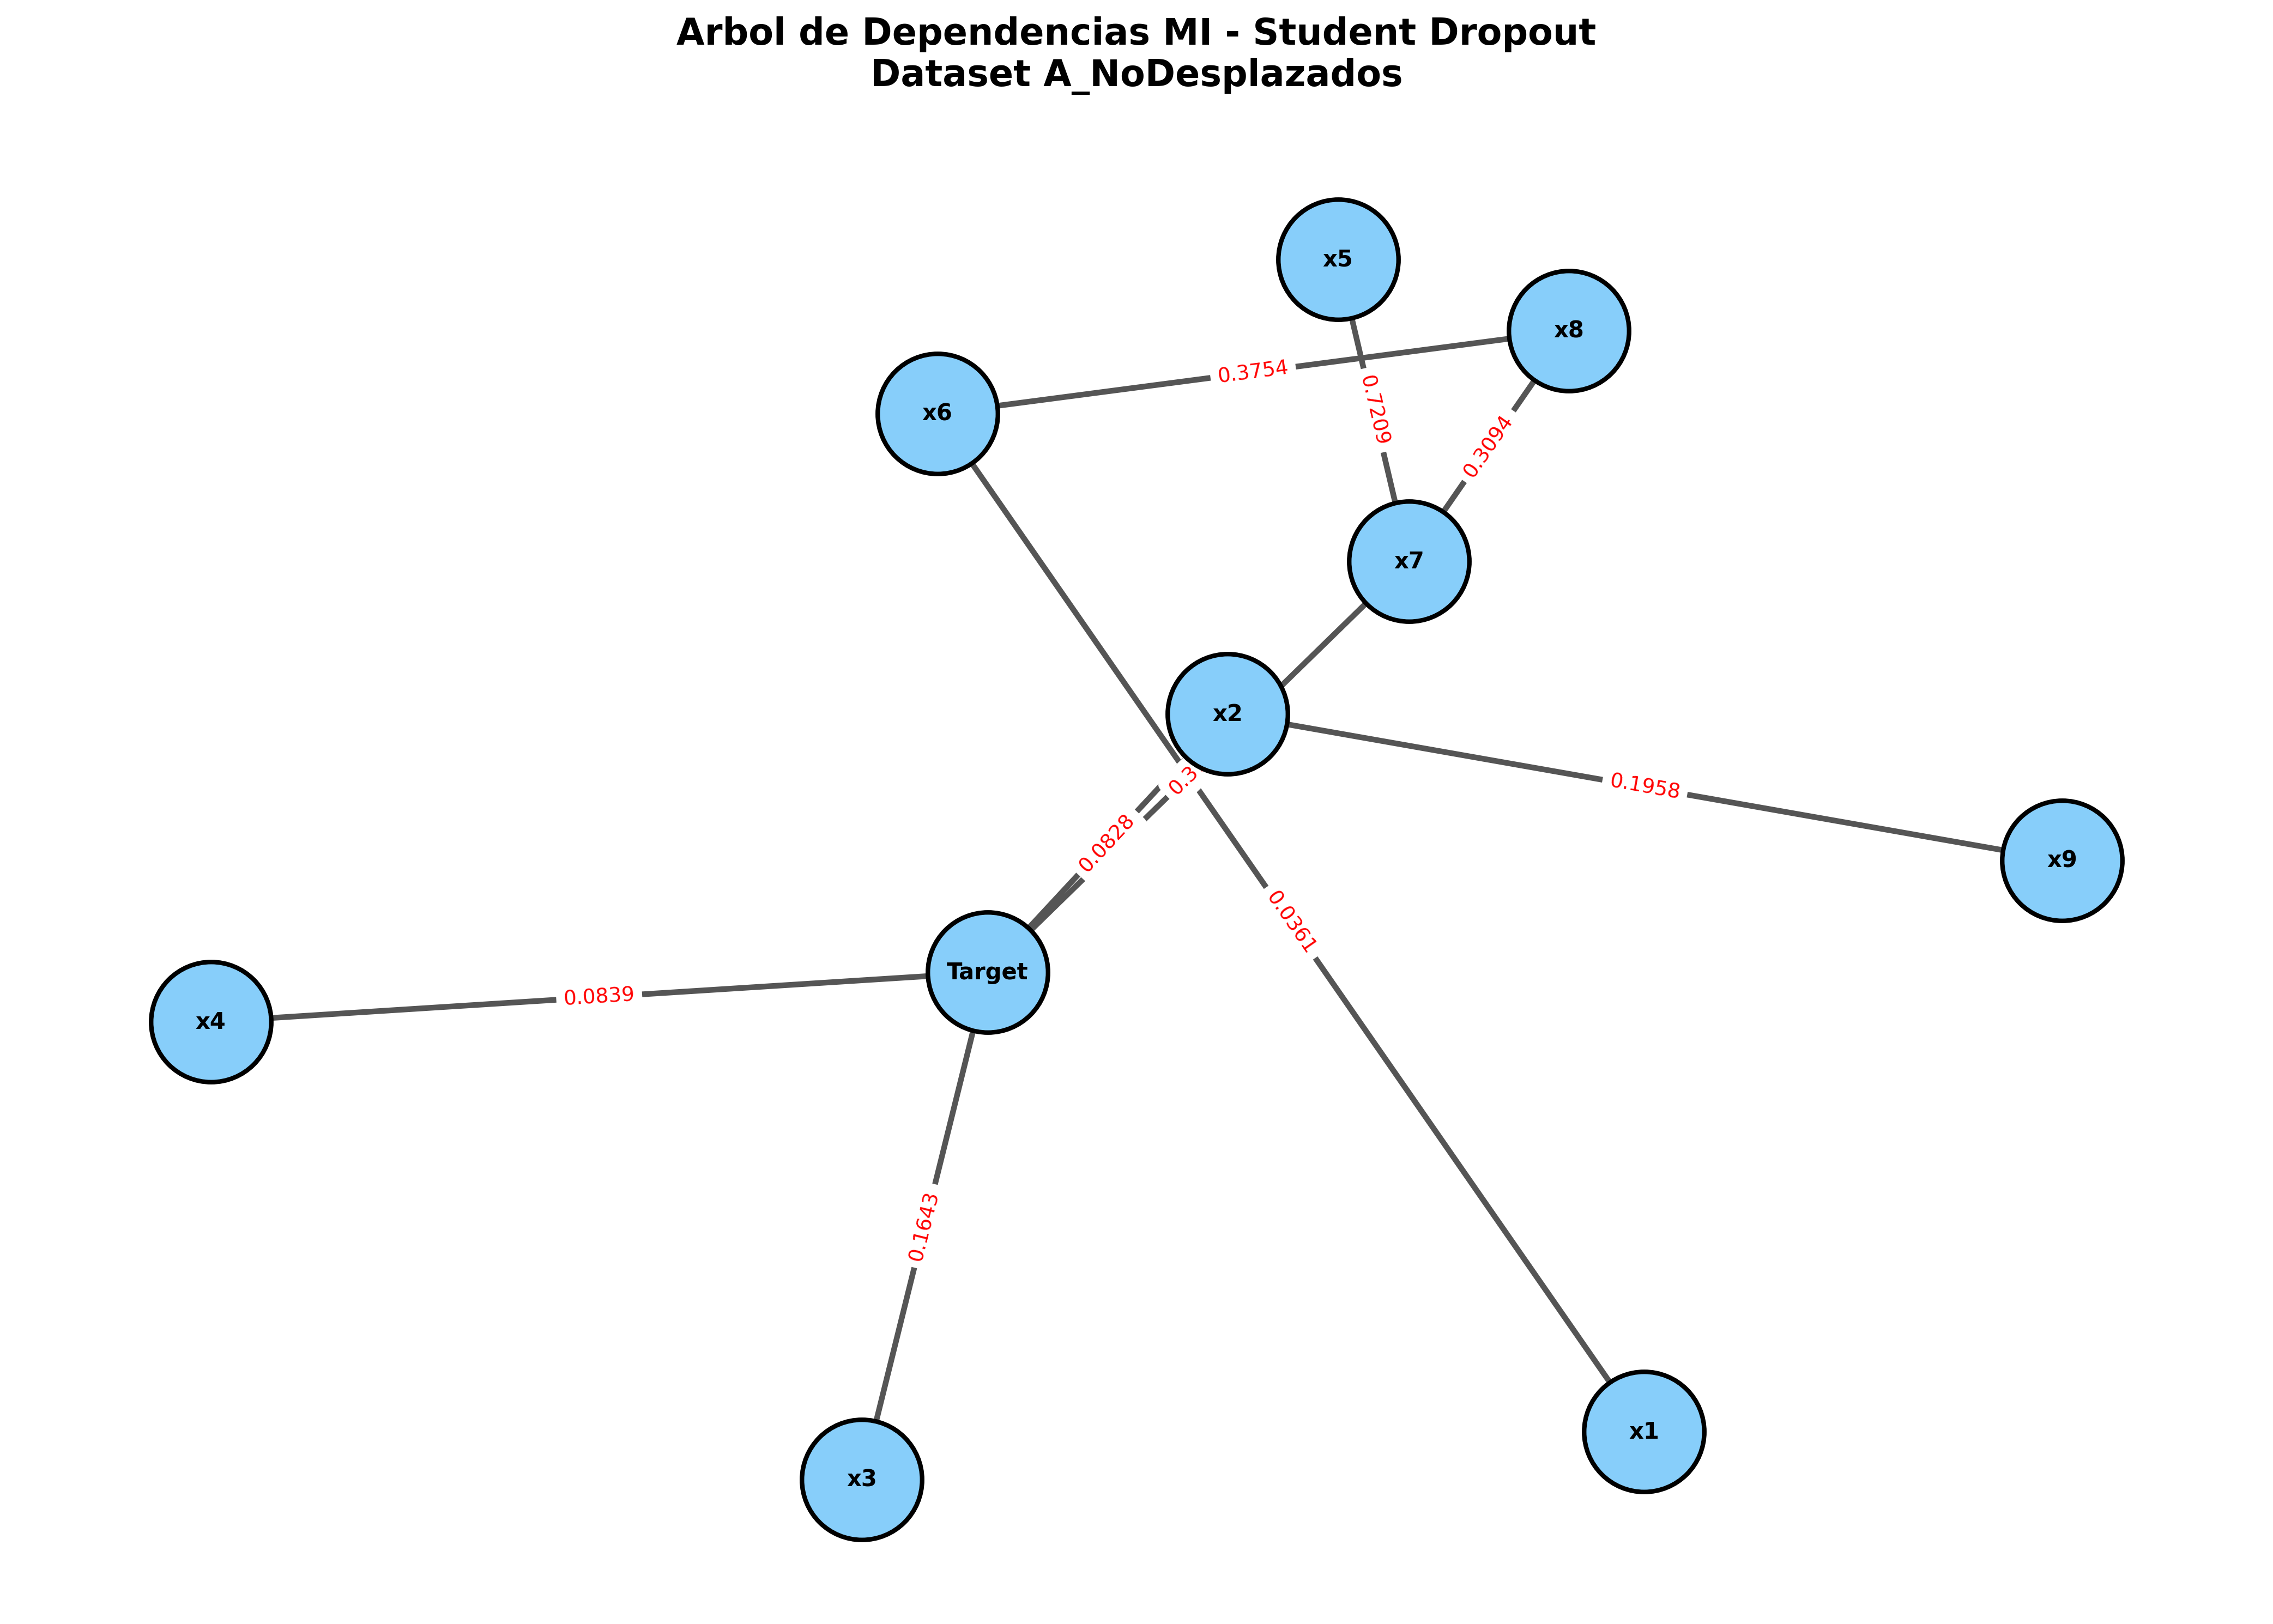
\includegraphics[width=0.85\textwidth]{arbol_A_NoDesplazados.png}
    \caption{Árbol de Expansión Máxima -- Dataset A (No Desplazados).}
    \label{fig:arbolA}
\end{figure}

\begin{figure}[H]
    \centering
    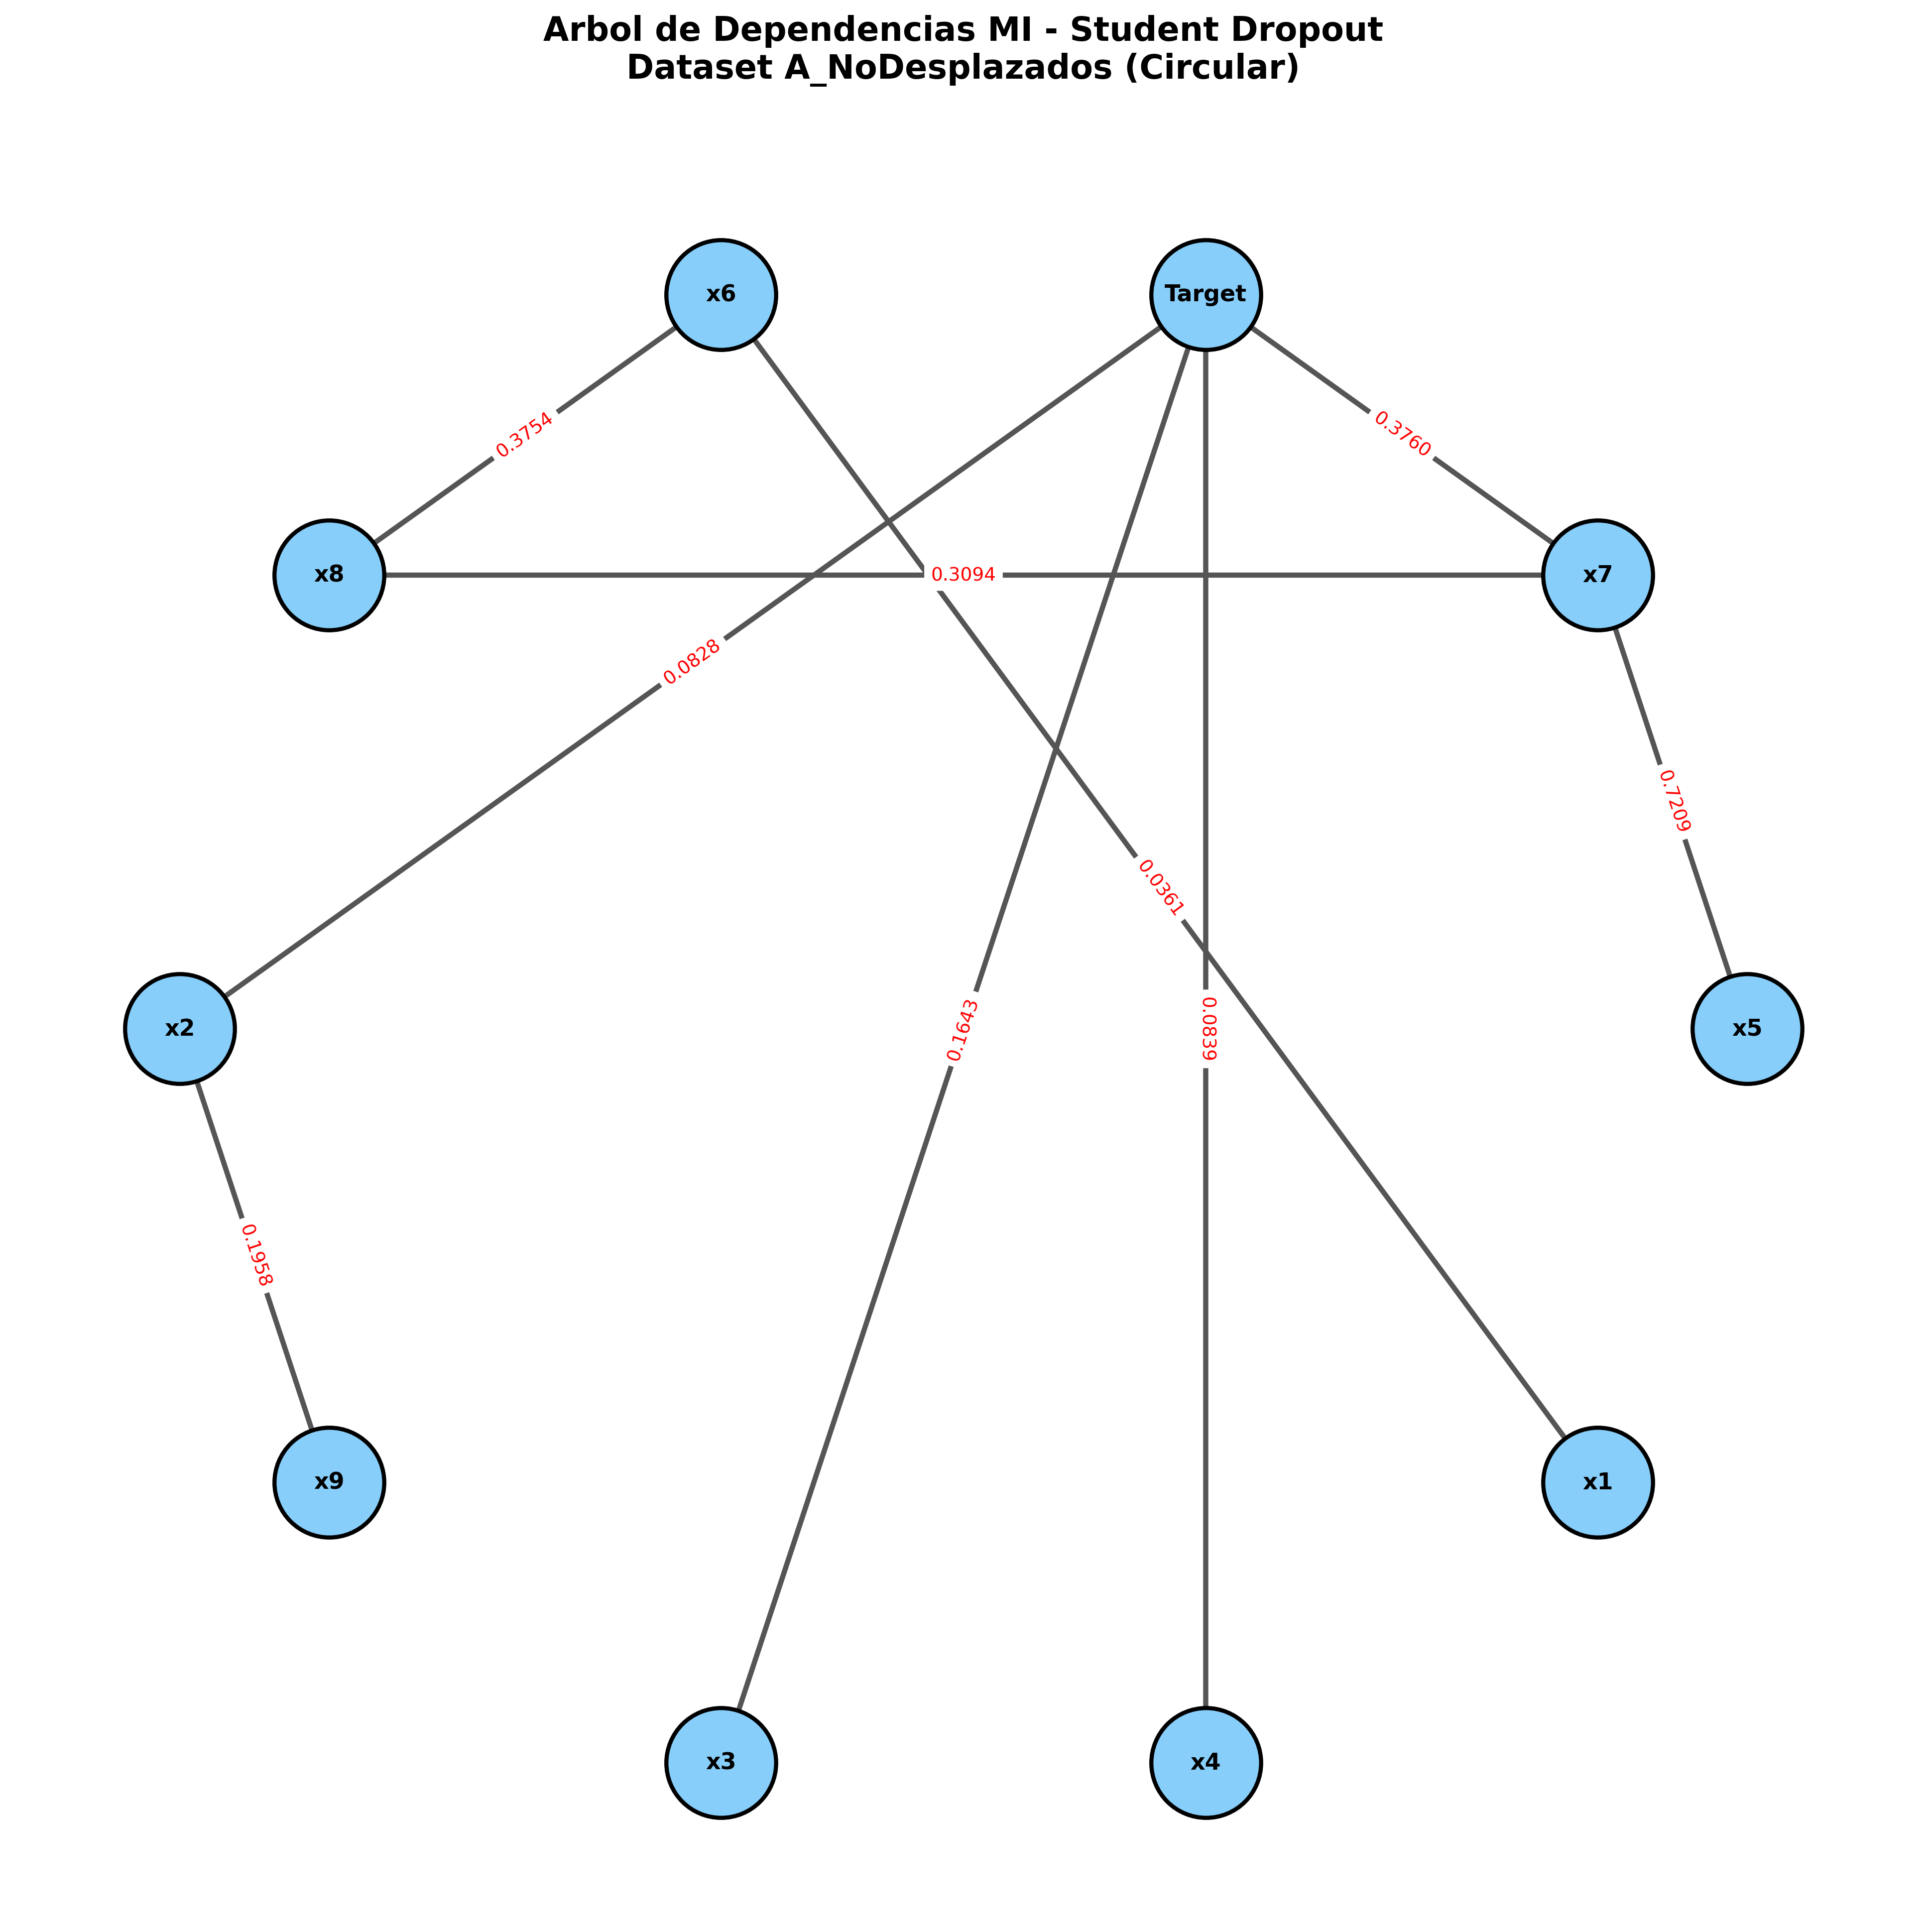
\includegraphics[width=0.75\textwidth]{arbol_A_NoDesplazados_circular.png}
    \caption{Distribución Circular del Árbol -- Dataset A (No Desplazados).}
    \label{fig:arbolA_circ}
\end{figure}

% =============================================
% DATASET B (DESPLAZADOS)
% =============================================
\newpage
\end{document}
